
%%%%%%%%%%%%%%%%%%%%%%%%%%%%%%%%%%%%%%%%%%%%%%%%%%%%%%%%%%%%%%%%%%%%
\section{DAQ Design}
\label{sec:fdsp-daq-design}

\metainfo{16 Pages}


%%%%%%%%%%%%%%%%%%%%%%%%%%%%%%%%%%%
\subsection{Overview (Giles Barr)}
\label{sec:fdsp-daq-ltr}

%Here we describe the overall readout and data acquistion
%strategy. This will include the high-level data flow diagram,
%(Figure~\ref{fig:daq-readout-buffering-baseline} may be sufficient)
%which is divided in functional boxes, each of which are described in
%turn in the sections below.

The design for the \dword{daq} has been driven by finding a cost
effective solution that satisfies the requirements. Several design
choices have nevertheless been made. 
From a hardware perspecive, the DAQ design follows a standard HEP
experiment design, with customised hardware at the upstream, feeding
and funnelling (merging) and moving the data into computers. 
Once the data and triggering information are in computers, a
considerable degree of flexibility is available and the processing
proceeds with a pipelined sequence of software operations, involving
both parallel processing on multi-core computers and switched
networks. The flexibility allows the procurement of computers and
networking to be done late in the delivery cycle of the DUNE
detectors, to benefit from increased capability of commercial devices
and falling prices.

Since DUNE will operate over a number of decades, the DAQ has been
designed with upgradability in mind.  With the fall in cost of serial
links, a guiding principle is to include enough output bandwidth to
allow all the data to be passed downstream of the custom hardware.
This allows the possibility for a future very-fast farm of computing
elements to accommodate new ideas in how to collect the DUNE data.  The
high output bandwidth also gives a risk mitigation path in case the
noise levels in a part of the detector are higher than specified and
higher than tolerable by the baseline trigger decision mechanism; it
will allow additional data processing to be added (at additional cost).

The data will be collected from the TPC and photon-detector readout
systems of the single-phase and dual-phase \dwords{detmodule}. 
These partitions are viewed as essentially four types of
\dwords{submodule} within the DAQ and will follow the same overall
data collection scheme as shown in figure 1. 
The readout is arranged in a hierarchical manner to allow localized
\dword{l0primitive} decisions to be made at the \dword{detunit} level,
at the cavern level before being combined over the full four caverns. 
The control of the detector elements will allow a fault in one part to
not halt data taking in another part, certainly at the per-cavern
level, but maybe also at more local levels. 
This will prevent a supernova burst following a failure in some part
of a cavern from being missed.

\metainfo{The folowing text will need considerable revision to make
  sure it corresponds with whatever ends up as figure 1, but the text
  here gives an idea that the overview will be a very quick visit of
  everything, and all the detail is in the later sections. 
  Note, migrated \textbf{boldface} terms to ``DUNE Words'' (bv).}

It is helpful, on first looking at the DUNE DAQ dataflow scheme, to
consider how the main data is collected first and then to look at how
the triggering and synchronization functions are included; we take
this approach in this overview. 
The main data are initially merged within one \dword{detunit} (eg, one
APA) and placed in a \dword{ringbuffer} to allow \dwords{trigdecision}
to be made. 
When a \dword{trigdecision} is performed it results in all data in a
determined time window and in a designated region of interest (ROI) as
specified by the \dword{trigcommand} to be extracted from the
\dword{ringbuffer} and sent for event building, \dword{diskbuffer} and
possible transfer to permanent storage at Fermilab. 
This covers trigger decisions for the purpose of collecting data
covering interactions of beam and atmospheric neutrino, cosmic rays,
individual supernova neutrinos and also candidates for searches such
as proton decays, or low energy events such as solar and diffuse
supernova neutrinos as well as sources of calibration. 
Additionally, when a supernova burst is detected internally within
DUNE, a further \dword{dumpbuffer} will be used to store all the data
for all APAs for a long period. 
The \dword{ringbuffer} must be long enough for trigger decision
latency (including the time for enough supernova events in a burst to
arrive and appear over the background). Further details of the
buffering scheme is described in section~\ref{sec:fdsp-daq-ltr}
% 7.2.2.

% want a \subsubsection here?
(Triggering Overview) In parallel with the data buffering scheme
described above, summaries of detected hits \dwords{l0primitive} are
assembled at the APA level to detect clusters of hits and apply
algorithms to distingush them from background (either radioactive
decays or detector noise). This is described in detail in
Section~\ref{sec:fdsp-daq-ltp}.
% 7.2.3. 
Whether this process is more suitable for FPGAs or computers is under
study, as it depends on the interfaces, both can be accomodated in the
architecture, and both have been costed. \fixme{neither yet!}
To retain the APA-level modulariy, the trigger primitives are
collected and processed in the same APA node that buffers the data.
The trigger primitives are then sent to the cavern level and then the
detector-level triggers to allow both multi-APA triggers to be formed
and also allow the supernova burst detection decisions to be made to
initate data transfer to \dword{dumpbuffer}. 
This is described in detail in Section~\ref{sec:fdsp-daq-sel}.
% 7.2.5. 
When a \dword{trigdecision} is formed, instructions are sent to the
\dword{ringbuffer} to retrieve the full data, build them into events
and store the results in the \dword{diskbuffer}.
The events for the main physics analyses will be retained for offline
study at this point in the DAQ. 
A software trigger algorithm could be run at this point to eliminate
obvious noise-source events (such as pickup on a row of wires),
especially if numerous. 
A further feature, useful for certain supernova studies will be to let
a sample of below-threshold events through to the secondary buffers
where they are retained for a few hours. 
If a SNEWS external warning of supernova is subsequently received,
these events can be kept permanently if desired, to allow lower
thresholds during a SNEWS period than normal.

(Synchronisation Overview) Unknown until the interface with elecronics is known

%%%%%%%%%%%%%%%%%%%%%%%%%%%%%%%%%%%
\subsection{Local Readout \& Buffering (Giles Barr \& Giovanna Miotto \& Brett Viren)}
\label{sec:fdsp-daq-ltr}

\metainfo{Describe how the data is received from the detector electronics, and buffered while awaiting a trigger decision, together with any processing that affects stored data.  The starting point is data incoming from the WIBs and the end point is corresponding data sitting in memory ready for event building. }

Figure~\ref{fig:daq-readout-buffering-baseline} illustrates the local
readout and buffering data flow in the context of a single APA.  

\begin{dunefigure}[Baseline Readout and Buffering]{fig:daq-readout-buffering-baseline}
  {Illustration of data flow for two out of 150 APAs in the
    Single-Phase module. 
    It shows the Cold Electronics WIB-RCE connections which send one
    half of one APA face to each RCE. 
    The data and L0 trigger primitives the RCEs are received by a
    single FELIX host. 
    The data is buffered into RAM and the trigger primitives are sent
    to the Module Trigger Logic unit (MTL) and sent to the Global
    Trigger Logic unit (not shown). 
    Nominal (non-dump) trigger commands are delivered to the Event
    Builder which polls the selector on the appropriate FELIX host for
    the requested data.
    The MTL sends special SNB-dump trigger commands directly to the
    Front-End Readout hardware so that it may initiate a full-stream
    dump to local storage. 
    This dump is then sent out over Ethernet to a special SNB Event
    builder. 
    Both types of event builders finally save triggered data to file
    on the offline buffer disk.}
% This PDF is made from the .dot of the same name.
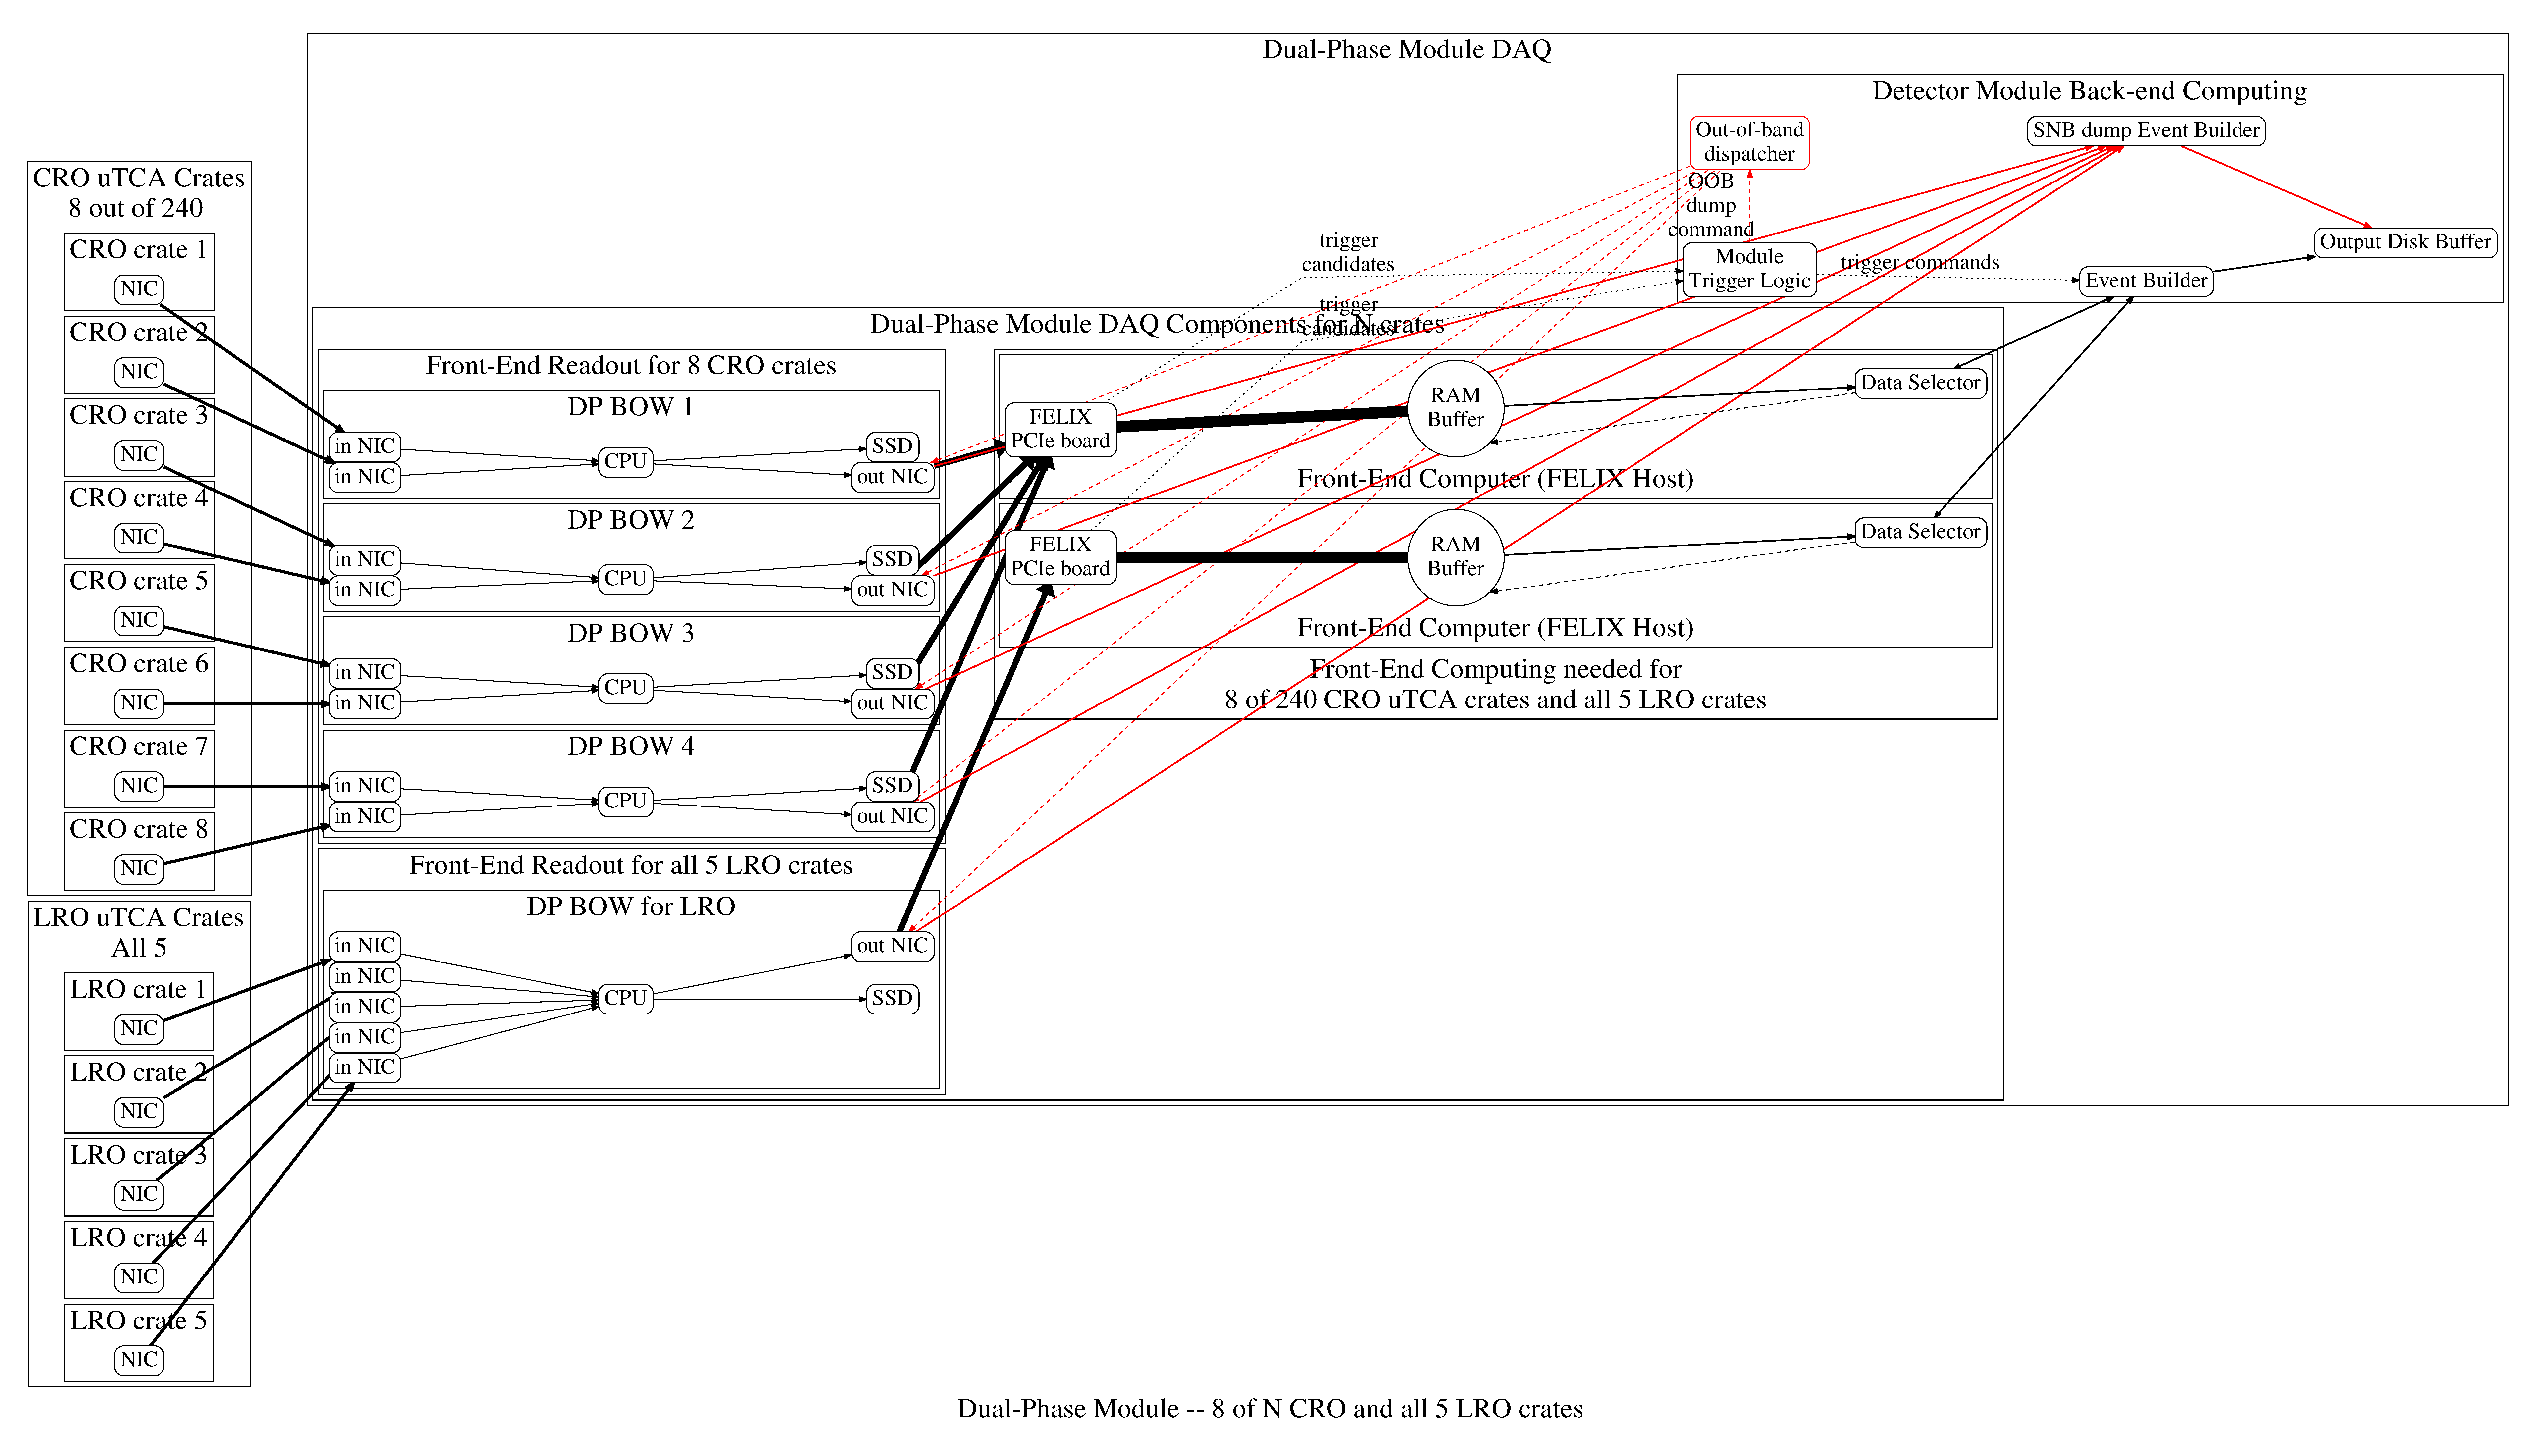
\includegraphics[width=0.8\textwidth]{daq-readout-buffering-baseline.pdf}%
\end{dunefigure}


%%%%%%%%%%%%%%%%%%%%%%%%%%%%%%%%%%%
\subsection{Local Trigger Primitive Generation (Josh Klein \& J.J. Russel \& Brett Viren \& DP Expert?)}
\label{sec:fdsp-daq-ltp}

\fixme{Below are from slides bv may show at the Jan WS.  Content copied here and now as a starting point.}

The TPC data is used to generate \textit{trigger primitive messages}
(TPM) local to each APA and which summarize the activity recently
sensed by their connected conductors.  These TPMs are emited from each
APA DAQ Front End and become fodder for later determining
\textit{trigger command messages} (TCM) as described in
Section~\ref{sec:fdsp-daq-sel}.

Only the 480 collection channels associated with each APA face are
used for forming TCMs.  Reasons for this reduction include the fact
that collection channels:

\begin{itemize}
\item have higher signal to noise ratio compared to induction channels.
\item fully and independently are sensitive to each APA face.
\item have unipolar signals that directly give an approximate measure
  of ionization charge without costly field response deconvolution
  computation.
\item can be divided into smaller groups defined by natural hardware
  boundaries for parallel processing.
  % fixme: do we need a statement about efficiency here?
\end{itemize}


Figure~\ref{fig:daq-overview} illustrates the connectivity between the
four connectors on each of the five WIBs and the DAQ APA Front End.
The data is received from 80 1 Gbps fiber optical links by four
Reconfigurable Computing Elements (RCE) in the ACTA Cluster On Board
(COB) system. \fixme{Matt: help!  Each RCE consists of a ....}

The pattern of connectivity between WIBs and RCEs results in the data
from the collection channels covering one half of one APA face being
received by each RCE.  Each RCE has two primary functions.  The first
is transmission of all data as described in
Section~\ref{sec:fdsp-daq-hlt}.  The second is to produce TPMs from
its portion of the collection channel data.

The TPMs are produced from a \textit{trigger primitive production
  pipeline} of algorithms.  These algorithms still require development
but can be broadly described.   

\begin{enumerate}
\item On a per channel basis calculate a rolling baseline and RMS that
  characterizes recent samples minimal influence from ionization
  signal.
\item Locate contiguous ADC samples that go above a threshold which is
  defined in terms of the baseline and RMS.
\item Emit their time bounds and total charge as a $ROI_{ch}$ TPM.
\end{enumerate}

These $ROI_{ch}$ TPM represent some possible activity occurring
somewhere in the LAr within a $\pm$\SI{2.5}{\mm} strip that extends in
time by the ROI time bounds.  Depending on the threshold set, these
TPMs may be numerous due to \Ar39 decays and noise fluctuations.
Further processing must be done with more global information.  This
may be done as part of the Module Trigger Logic (MTL) as described in
Section~\ref{sec:fdsp-daq-sel} or it may be done immediately in the
RCE pipeline.  Strategies to summarize these detailed TPM into fewer
TPMs include:

\begin{enumerate}
\item Pad each $ROI_{ch}$ in a channel by a fixed amount in order to
  anticipate their use later as defining readout (eg, long enough to
  account for inter-plane drift times (\SI{6.25}{\micro\second}) and
  induction signal extents ($\sim$\SI{100}{\micro\second}).
\item Form the union of ROI across all channels observed by a given RCE.
\item Merge subsequent ROI which are separated by some small time
  interval.
\end{enumerate}

If the Single-Phase detector module generates excess noise, such as
that from RF emission picked up coherently across some group of
channel, it must be mitigated at the start of the pipeline and will
likely require additional computational resources.  Some ideas to
respond to this scenario include....\fixme{Ideas?}.



%%%%%%%%%%%%%%%%%%%%%%%%%%%%%%%%%%%
\subsection{Dataflow, Trigger and Event Builder (Giles Barr \& Josh Klein \& Giovanna Miotto \& Kurt Biery \& Brett Viren)}
\label{sec:fdsp-daq-hlt}

\metainfo{Describe the dataflow {\it infrastructure}. This should cover transport of data and trigger information, infrastructure for generating local and global trigger commands (but not their algorithms, that's next), as well as what happens to the data once a trigger is generated (ie. event building).
Figure~\ref{fig:daq-readout-buffering-baseline} may be referenced}

The data volume that is flowing around the DUNE DAQ is considerable,
over 10TB/s conntinuoiusly.  However, the control of it is simplified
by making the modularity of the {\bf primary buffer} at the APA level.
The majority of the data corresponds to the untriggered parts and
never leaves the nodes that house the primary buffers.  The parts that
do exit in one of three circumstances, (a) as selectd {\bf event} data
(b) as trigger primitives, to be considered on the cavern-wide
decision step or (c) as previously triggered supernova burst data
being 'trickled out' from the SSD storage.  All thee of these
transfers lives entirely in the software domain of a commodity
computer farm and so a variety of techniques can be considered for
each; in this description, we consider each of them as a data-pull
protocol, similar to that in use at ProtoDUNE.

artDAQ is a modern, general-purpose framework, that has been used in
DUNE prototype tests and elsewhere [refs].  It is optimised further
than other frameworks to expliot the paralelism that is possible with
modern multi-core machines.  It is the principle architecture that
will be used in DUNE. The authors of artDAQ have accomodated
DUNE-specific feature-addition requests, an a number of libraries have
been used by linking into the 'boardreader' parts of artDAQ (the parts
that handle the incloming data from the data sources), and it is
likely that future DUNE extensions will be by one of these two routes.

(Section on FELIX data ingress, error handling, synchronisation,
ring-buffer expiry).  As noted above, one of the complex data flow
control tasks is managing the data asit enters the {\bf primary
  buffers} on the {\bf per-APA nodes}.  Data throughput on these nodes
is governed by the use of the PCIe and memory busses, and so the
softwre will be written to mimumize data-copies on the input side of
the {\bf primary buffer}.  During normal operation, there must be
sufficient 'headroom' to allow an additional write of data to SSDs
during the supernova burst.  The current model for dataflow control is
tht each APA will operate autonomously, data being written directly
from hardware into physical memory and not moved.  The softare will
keep track of the free and in-use memory (one way is with a ring for
each data source) and will maintain an index of the data.  One
strategy that decentralises the error handling is for the writing to
the {\bf primary buffer} to not cause error handling events, but for
it to flag areas of the data for which problems exist only if/when it
is to be read again.  Similarly to avoid memory alloction error
handling, the incoming data can overwrite the older data and read
requests for data that has been overwritten will report the error.  It
is planned to prototype the data transfers for the TDR.

(Section on (a) event building) Requsts for event building
(i.e. reading data for succesful triggers from the {\bf primary
  buffers} will be donw using mostly standard features that are now in
artDAQ.  An event-builder node is allocated for each trigger to be
read.  This event builder then requests portions of data from the {\bf
  primary buffers} for the data from that event (this read must be
initiated by the request, a difference with the current ProtoDUNE).
If the data is missing (either due to errors when it was first
received, or because the request arrived so late, that the data were
overwritten), the request proceeds, but with flags set in the event
header which are displayed on the operators console.

(Section on (b) trigger farming) The {\bf per-APA-node} will receive,
or generate the trigger primitives that summarise the hits from each
APA, organised in blocks of time.  In some circumstances, this is
sufficient to declare a trigger, in others, the hit pattern must be
combined between APAs to make the trigger decision.  The list of
APA-level decisions and the trigger primitives are assembled into a
block for each time block.  Our default scheme for the dataflow is to
use a similar method to PotoDUNE, however several others are under
study.  In the ProtoDUNE method, a trigger farm node is assigned to
each time block and requests the trigger data block for it.  When it
receives the data from all the APAs, it builds an event (using artDAQ
funcions), and then processes it, to assign the trigger decisions.
One alternative (to avoid the possibility that too many small blocks
of data must arrive in one place at a time) is to split the cavern
into regions, and have an intermediate layer of data collecton.
Another solution is to use data-push, since, it is likely that a
single node with a lot of cores can deal with all the trigger
processing.

(Section on (c) SNB trickling) Because of the ling-term storage
capabilities of the SSD drives, there is no hurry to colect the data
from them for a supernova.  This task can therefore be done in the
background (indeed, it should be halted during a subsequent SNB
trigger, to avoid increasing the data transfers in the per-APA node).
It is anticipated that a spernova collecor node will use data-pull
requests to slowly collect the data from each node and merge it in
some way for offline analysis.  Probably there will be one data file
per APA node which will be collected together in a directory;
presumably the offline will not want a single 10TB long file.


%%%%%%%%%%%%%%%%%%%%%%%%%%%%%%%%%%%
\subsection{Data Selection Algorithms (Josh Klein \& Brett Viren)}
\label{sec:fdsp-daq-sel}

%This section describes the strategy for using the trigger/dataflow infrastructure, with example algorithms.

	Data Selection will follow a hierarchical design, beginning with local,
APA Level trigger candidates, Module (10 ktonne) Level triggers, and Global
(Detector-wide) triggers. A high-level trigger (HLT) may also be active within
the Module Level trigger.  The hierarchical approach is both natural from a
design standpoint, as well as allowing for vertical slice testing and
partitioning during commissioning of the system.

	As discussed above, trigger primitives will be generated in the RCEs
from the data stream for each collection wires.  The trigger primitives will be
summary information for each collection wire, such as the time of any
threshold-crossing pulse, its integral charge, and time over threshold.  A
collection wire with a non-null trigger primitive is said to be ``hit.''  These
trigger primitives are then passed, along with the full data stream, to the
FELIX boards and their hosts, each of which handles channels from a small
number of APAs (likely two).  An APA Level trigger candidate is passed upward to
a Module Level trigger, which arbirtrates between various trigger types,
determining whether a given APA Level trigger candidate is a valid Module
Trigger and whether there are other triggers that have a higher priority in any
given slice of time.  At this level, a more sophisticated high-level trigger
(HLT) may also be employed, which will allow a reduction in trigger rate from
various backrounds, including instrumental backgrounds, if needed. 

	A valid Module Level single-interaction trigger sends trigger commands
back to the FELIX hosts telling them which slice of time should be saved under
the particular trigger header.  At the start of DUNE data taking, it is
anticipated that for any given single-interaction trigger (a cosmic ray track,
for example) waveforms for all wires will be recorded for a full 5.4~ms
``readout window.'' Such an approach is clearly very conservative, but it
ensures that associated low-energy physics (such as neutron captures from
neutrons produced by neutrino interactions or cosmic rays) will be recorded
without any need to fine-tune APA-level triggering, and will not depend on
the noise environment across the APAs. In addition, the 5.4~ms readout window
ensures that regardless of when a given even causes a trigger, the entire track
is recorded.  We anticipate, however, that as we gain experience running DUNE
the overall data volume will reduced by writing out data from only a
subset of APAs for any given track, and possibly reducing the size of the
readout window.

	Other trigger streams---calibrations, random triggers, and prescales of
various trigger thresholds, will also be generated at the Module Level, and
filtering and compression can be applied based upon the trigger stream. For
example, a large fraction of random triggers may have their waveforms
zero-suppressed, reducing the data volume substantially, as the dominant data
source for these will be $^{39}$Ar events. Additional signal-processing can
also be done on particular trigger streams if needed and if the processing is
available, such as fast analyses of calibration data.

       At the Module Level, a decision can also be made on whether a series of
interactions are consistent with a supernova burst.  If the number of APA Level
low-energy trigger candidates exceeds a threshold for the number of such events
in a given time, a trigger command is sent from the Module Level back to the
RCEs, which store up to 10 seconds of unsuppressed, full waveform data.  That
full waveform is then written out as a separate trigger stream for fast
analysis by the supernova working group, perhaps as an automated process.  In
addition, the Module Level passes information about APA Level trigger
candidates  up to a detector-wide Global Trigger, which can decide whether,
integrated across all modules, enough APAs have detected interactions to
qualify for a supernova burst even if within a particular module the threshold
is not exceeded. Trigger commands from the Global Trigger Level are passed
downward to RCEs in the same way as any Module Level supernova burst trigger
would be; at the Module Level, a Global Trigger looks like just one more
``external'' trigger input.

	APA Level trigger candidates will be generated within each FELIX
host.  The trigger decision will be based on the number of adjacent wires hit
in a given APA within a narrow time window (roughly 100$\mu$s), the total
charge on these adjacent wires (or any wire with a non-null trigger primitive),
and possibly the time-over-threshold for collection wires with hits. Our
studies show that even for low-energy events (roughly 10-20 MeV) the reduction
in radiological backgrounds is extremely high with such criteria. The
highest-rate background, $^{39}$Ar, which has a decay rate of 10 MBq within a
10 ktonne volume of argon, has an endpoint of 500 keV and requires significant
pileup in both space and time to get near a 10 MeV threshold. Other important
background sources are $^{42}$Ar, which has a 3.5 MeV endpoint and a decay rate
of 1 kBq, and $^{222}$Rn which has a decay rate of XXXX and decays via a
highly-quenched $\alpha$ of 5.5 MeV.  The radon decays to $^{218}$Po which
a few minutes later leads to a quenched $\alpha$ of 6 MeV, and ultimately a
$^{214}$Bi daughter (many minutes later) which has a $\beta$ decay with
endpoint near 3.5 MeV.  The $\alpha$ ranges are short and will hit at most a
few collection wires, but the charge deposit can be large, and therefore the
charge threshold will have to be well above the $\alpha$ deposits plus any
pileup from $^{39}$Ar and noise.

	At the APA Level, two kinds of local trigger candidates can be
generated. One is a ``high-energy'' trigger, that indicates that within a given
APA a candidate event with energy more than 10 MeV has been found. The
thresholds in hit wires, total charge, and time-over-threshold, will be
optimized for at least 50\% efficiency at this threshold, with efficiency
increasing to 100\% via a turn-on curve that ensures at least 90\% efficiency
at 20 MeV.  A second APA Level trigger candiate will be generated for
low-energy events, between 5~MeV and 10 MeV. These low-energy APA trigger
candidates will not by themselves generate valid  Module Level triggers, but
rather be used at the Module Level to determine whether a burst of events
across many APAs is consistent with a supernova.

	The Module Level takes as input both APA Level trigger candidates (both
low-energy and high-energy), as well as external trigger candidate sources,
such as the Global (detector-wide) trigger, external triggers such as SNEWS,
and information about the time of a Fermilab Beam spill.  The Module Level will
also generate internal triggers, such as random triggers and calibration
triggers (for example, telling a laser system to fire at a prescribed time).
In addition, at the Module Level prescales of all trigger types that normally
would not generate a Module Level will be made. For example, a single
low-energy trigger does not cause a Module Level trigger on its own, but at
some large prescale fraction it could be accepted.



	The Module Level is responsible also for checking candidate triggers
against the current Run Control trigger mask: in some runs, for example, we
may decide that only random triggers are accepted, or that certain APA trigger
candidates should not be accepted because those APAs are noisy or misbehaving
in some way.  In addition, the Module Level will count low-energy trigger
candidates from the APAs and, based upon the number and distribution of those
triggers in a long time interval (e.g., 10 seconds), decide to generate a
supernova burst trigger command. The trigger logic for a supernova burst will
be optimized to accept at least 90\% of all Milky Way supernovae, and our
studies of simple low-energy trigger criteria show that we can likely do much
better than that.  

	The HLT can also be applied at this level, particularly if there are
unexpectedly higher rates from instrumental or low-energy backgrounds, that
require some level of reconstruction or pattern recognition.  An HLT might also
allow for efficency triggering on lower-energy single interactions, or allow
for better sensitivity for supernovae beyond the Milky Way, by employing a
weighting scheme to individual APA Level trigger candidates---higher-energy
trigger candidates receiving higher weights. Thus, for example, two APA Level
trigger candidates consistent with 10 MeV interactions in 10 seconds might be
enough to create a supernova burst candidate trigger, while 100 5 MeV APA Level
trigger candiates in 10 seconds might not. Lastly, the HLT can allow for
dynamic thresholding; for example, if a trigger appears to be a cosmic-ray
muon, the threshold for single interactions can be lowered (and possibly
prescaled) for a short time after that to identify spallation products. In
addition, the HLT could allow for a dynamic threshold after a supernova burst,
to extend sensitivity beyond the 10 s readout buffer, while not increasing the
data volume associated with supernova burst candidates linearly. 

All low-energy trigger candidates are also passed upwards to the Global trigger
level, which can integrate the APA level trigger across all 10 ktonne modules
and determine if enough APAs have trigger candidates that a supernova burst may
be occuring. This approach increases the sensitivity to trigger bursts by a
factor of four (for 40 ktonnes), thus extending the burst sensitivity to a
distance twice as far as for a single 10 ktonne module. 

	The Module Level is also responsible for creating a trigger header that
includes a global timestamp for the trigger, and information on what type of
trigger was created. A log of all APA Level trigger candidates will also be
kept, whether or not they are part of a Module Trigger.  A

s described above, for any high-energy APA Level trigger candidate, a Module
Level trigger command is sent  to all FELIX hosts instructing them to save a
5.4~ms readout window will written for all wires across all APAs 
(providing the start and end times to the FELIX hosts).  Thus, a DUNE ``event''
is 5.4~ms of data from all wires in response to a Module Level trigger.  The
Module Level trigger is also responsible for sending the trigger commands that
tell the RCEs to dump their 10 s unsuppressed ``supernova'' buffer.  If a
supernova burst trigger is created at the Global trigger level, a trigger
command is passed back down to the Module Level, which then passes that on to
the RCEs for readout of the long (10 s) unsuppressed buffer, the same way it
would if a supernova burst is detected at the Module Level. 

	


%\metainfo{Describe Module Trigger Logic and Global Trigger Logic.
%  Describe creation of Trigger Command Messages (TCM) from TPMs.
%  Included external sources of TPMs such as SNEWS, Fermilab Beam,
%  testing triggers, periodic triggers, calibration triggers.}
%
%\metainfo{Here should go the assumptions that went into the thinking
%  for Josh's event category data volumes.  It can include discussion
%  of tighter selection criteria for ``cosmics'' such as Phil's
%  distribution of number of APAs hit by cosmics and arguments for
%  something less than 2+ drift time readouts.}

%
% %%%%%%%%%%%%%%%%%%%%%%%%%%%%%%%%%%%
% \subsection{High-Level Trigger}
% \label{sec:fdsp-daq-eb}
%
% Data selection after event building.
%

\subsection{Timing \& Synchronization (David Cussans \& Kostas Manolopoulos)}
\label{sec:fdsp-daq-timing}

%Describe the generation of timing/synchronisation signals and and distribution to the detectors.

All components of the DUNE Single Phase detectors are synchronized to
a common clock. In order make full use of the information from the
photon detection system the common clock must be aligned within a
single detector with an accuracy of O(1ns). In order to form a common
trigger for super novae between detector modules the timing between
detectors must be aligned with an accuracy of O(1ms). However, a
tighter constraint is the need to calibrate the common clock to
universal time (derived from GPS) in order to adjust the data
selection algorithm inside an accelerator spill, which requires an
absolute accuracy of O(1us).

Single and Dual phase detector modules use a different timing system,
driven by the different technical requirements and development history
of the two systems. A single phase detector module has many more
timing end-points than a dual phase module and many of the end-points
are simpler than the end-points in the dual phase, for example a WIB
vs. uTCA crate. Both systems have been sucessfully prototyped.

The DUNE Single Phase detectors use a development of the protoDUNE
timing system. Synchronization messages are transmitted over a serial
data stream with the clock embedded in the data. The format is
described in DUNE DocDB-1651. Figure \ref{fig:daq-readout-timing}
shows the overall arrangement of components within the Single Phase
Timing System(SPTS). A stable master clock, disciplined with a 10MHz
reference is used in the SPTS. A one-pulse-per-second (1PPS) signal is
also received by the system and is time-stamped onto a counter clocked
by the SPTS master clock, however the periodic synchronization
messages distributed to the Single Phase detectors are an exact number
of clock cycles apart even if there is jitter in the 1PPS signal.

The GPS signal is encoded onto optical fibre and transmitted to the
CUC, where it is converted back to an RF signal on coaxial cable and
used as the input to a GPS displined oscillator. The oscillator module
also houses a IEEE 1588 (PTP) Grand Master and an NTP server. The PTP
Grand Master provides a timing signal for the Dual Phase White Rabbit
timing network. The NTP server provides an absolute time for the 1PPS
signal. The SPTS relates its time counter onto GPS time by
timestamping the 1PPS signal onto the SPTS time counter and reading
the time in software from the NTP server.

The latency from the GPS antenna on the surface to the GPS receiver in
the CUC will be measured by optical time domain reflectometry at
installation. Given the modest absolute time accuracy required
(sufficient to select data within an accelerator spill) dynamic
monitoring of this delay is not required.

The White Rabbit synchronization signals from the Dual Phase are
time-stamped onto the SPTS clock domain and the SPTS synchronization
signals are time stamped onto the Dual Phase clock domain. This allows
the timing in the Single Phase and Dual Phase detectors to be
aligned. A similar scheme is used to relate the Single Phase protoDUNE
Single Phase timing domain to be related to the beam instrumentation
White Rabbit time domain.

In order to provide redundancy, and also the ability to easily detect
issues with the timing path, two independent GPS systems are used. One
with an antenna at the head of the Yates shaft, the other with an
antenna at the head of the Ross shaft. The two independent timing
paths are brought together in the same rack in the CUC. Using 1:2
fibre splitters one SPTS unit can be left as a hot-spare while the
other is active. This also allows testing of new firmware and software
during comissioning without the risk of loosing the SPTS if a bug is
introduced.


\begin{dunefigure}[Arrangement of Components in DUNE Timing System]{fig:daq-readout-timing}
  {Illustration of the components in the DUNE Timing System.}
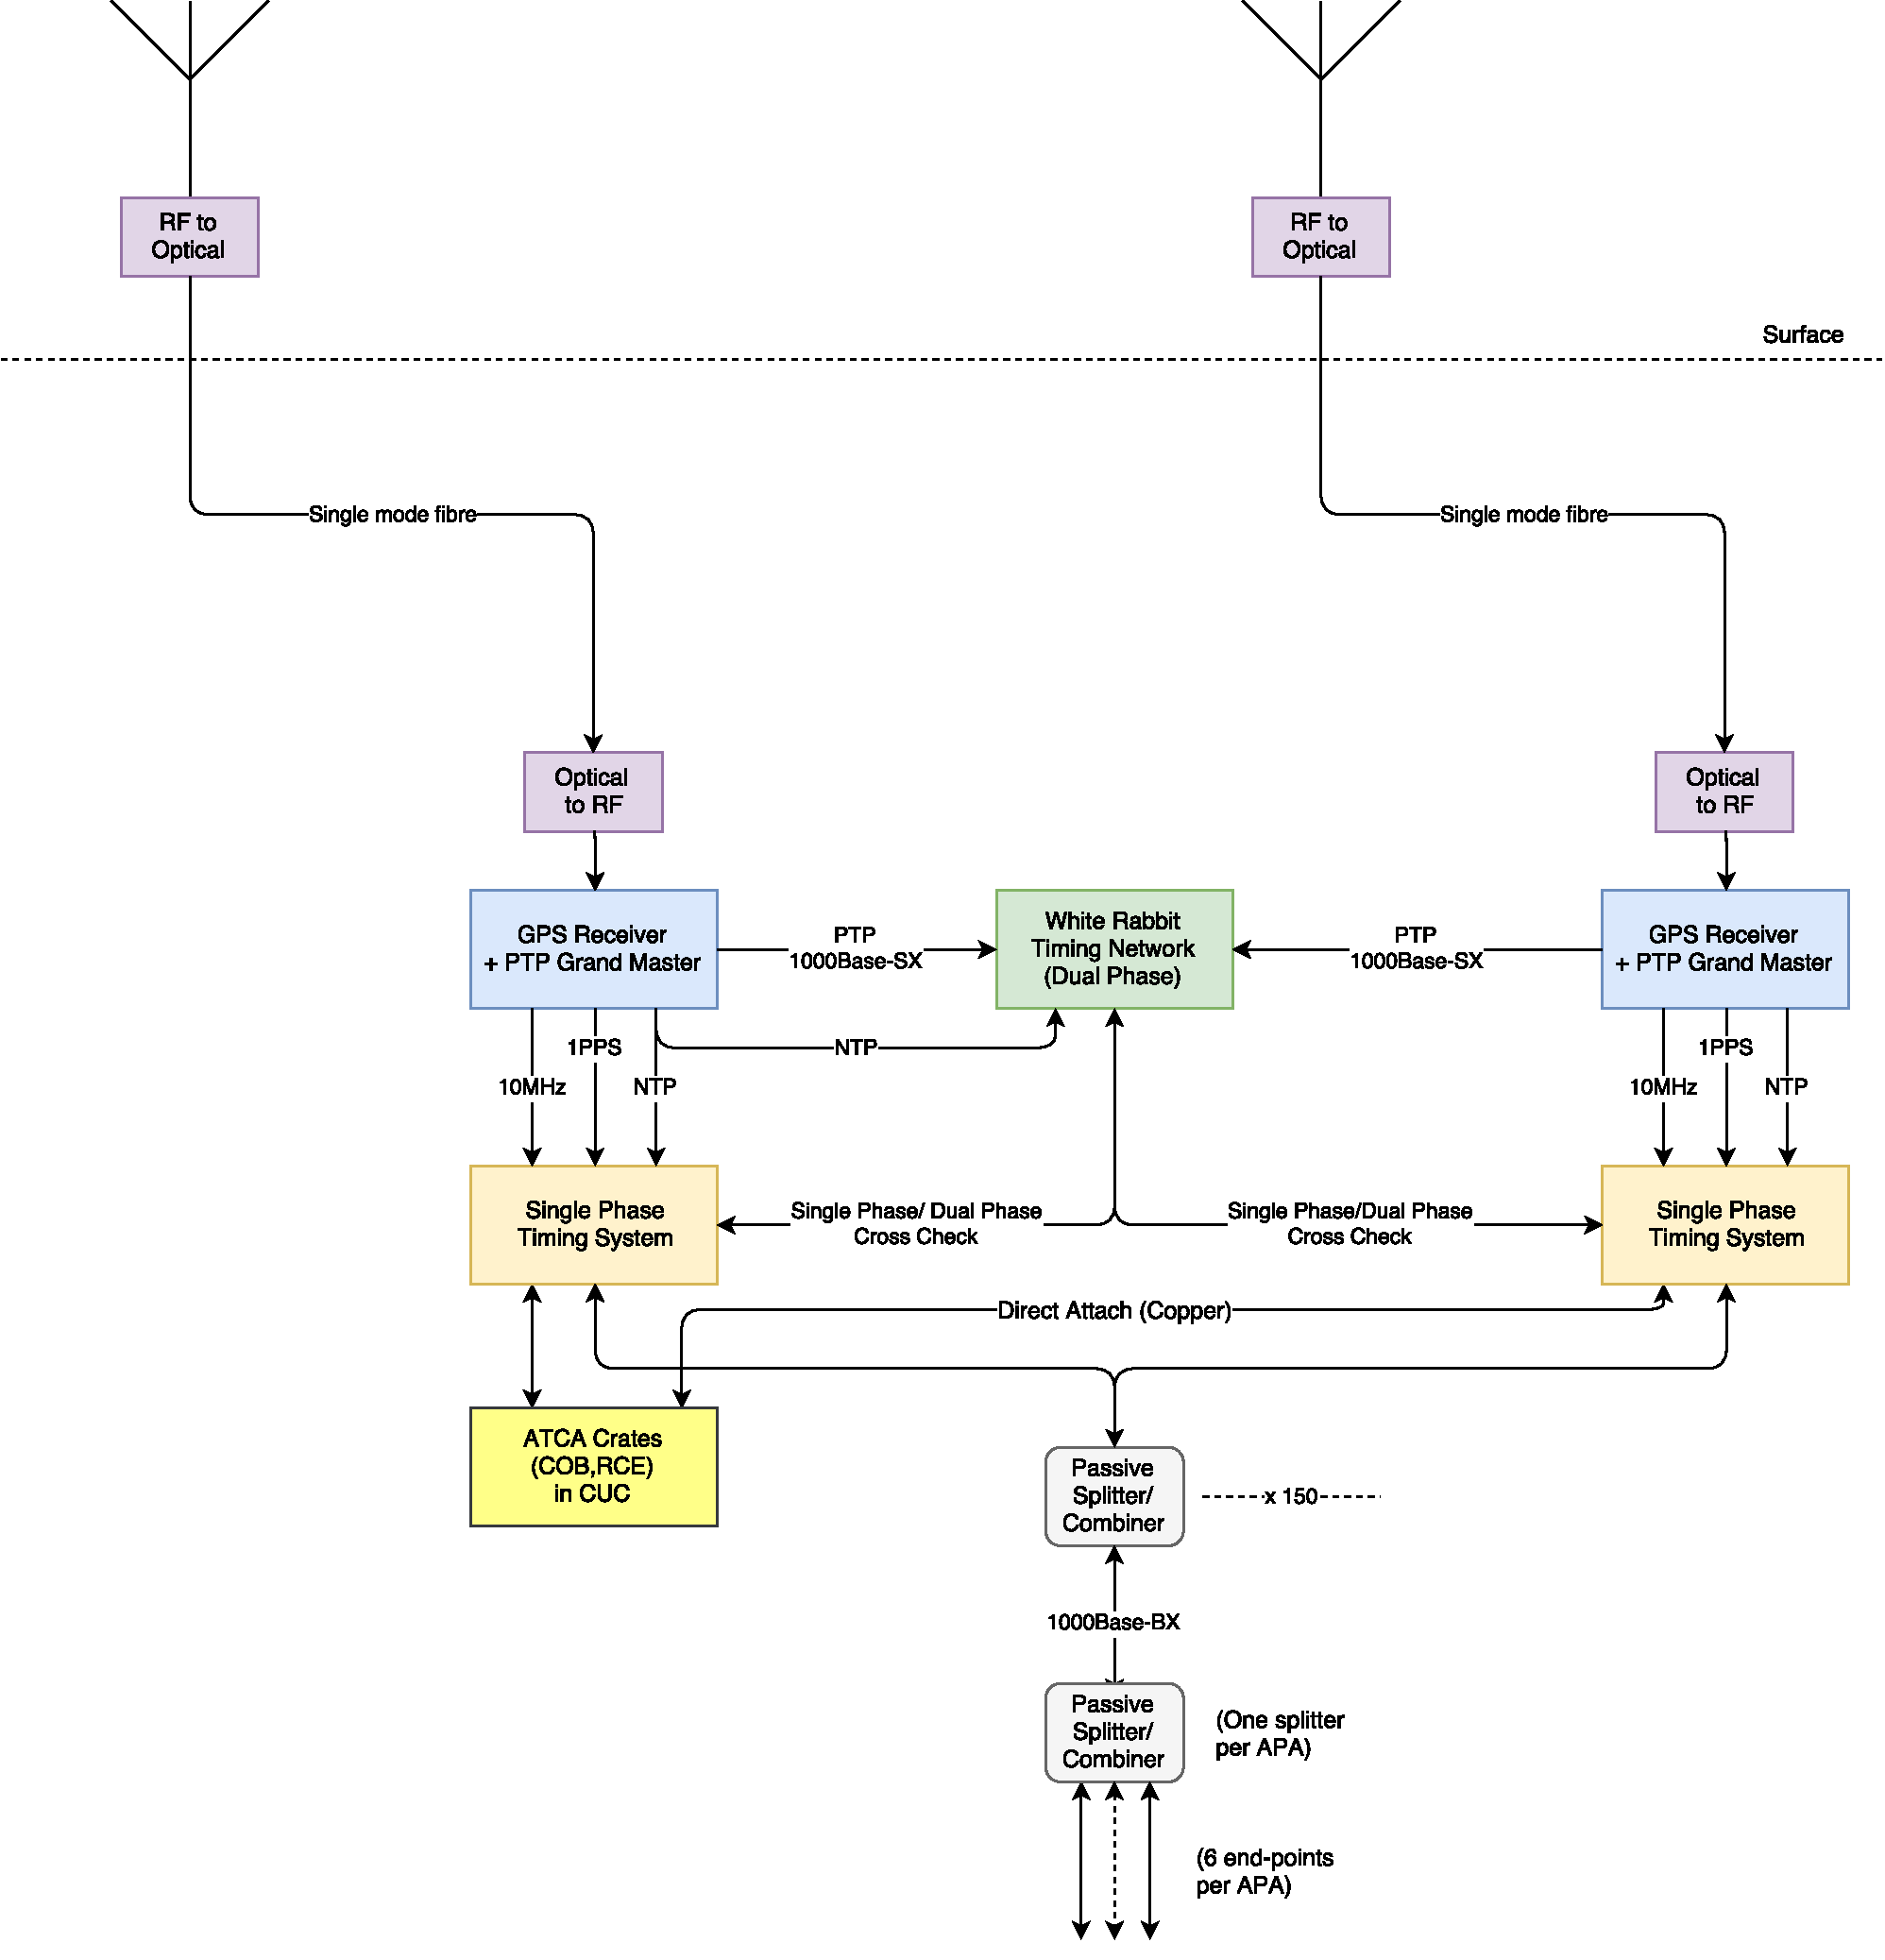
\includegraphics[width=0.8\textwidth]{DUNE_Timing_overall.pdf}
\end{dunefigure}

All the custom electronic components for the SPTS are contained in two
Micro-TCA shelves. At any one time one is active and the other is a
hot-spare. The 10MHz reference clock and the 1PPS signal are received
by a single width AMC at the centre of the Micro-TCA shelf. This
master timing AMC produces the SPTS signals and encodes them onto a
serial data stream. This serial datastream is distributed over a
standard star-point backplane to the fanout AMCs which each drive the
signal onto up to 13 SFP cages. The SFP cages are either occupied by
1000Base-BX SFPs, each of which connects to a fibre running to an APA,
or to a Direct Attach cable which connects to systems elsewhere in the
CUC, i.e. the RCE crates and the data selection system. This
arrangement is shown in figure \ref{fig:daq-readout-sp-timing}


\begin{dunefigure}[Arrangement of components in Single Phase Timing System]{fig:daq-readout-sp-timing}
  {Illustration of the components in the Single Phase Timing System.}
  %\fixme{Add a diagram of the SPTS electronics}
  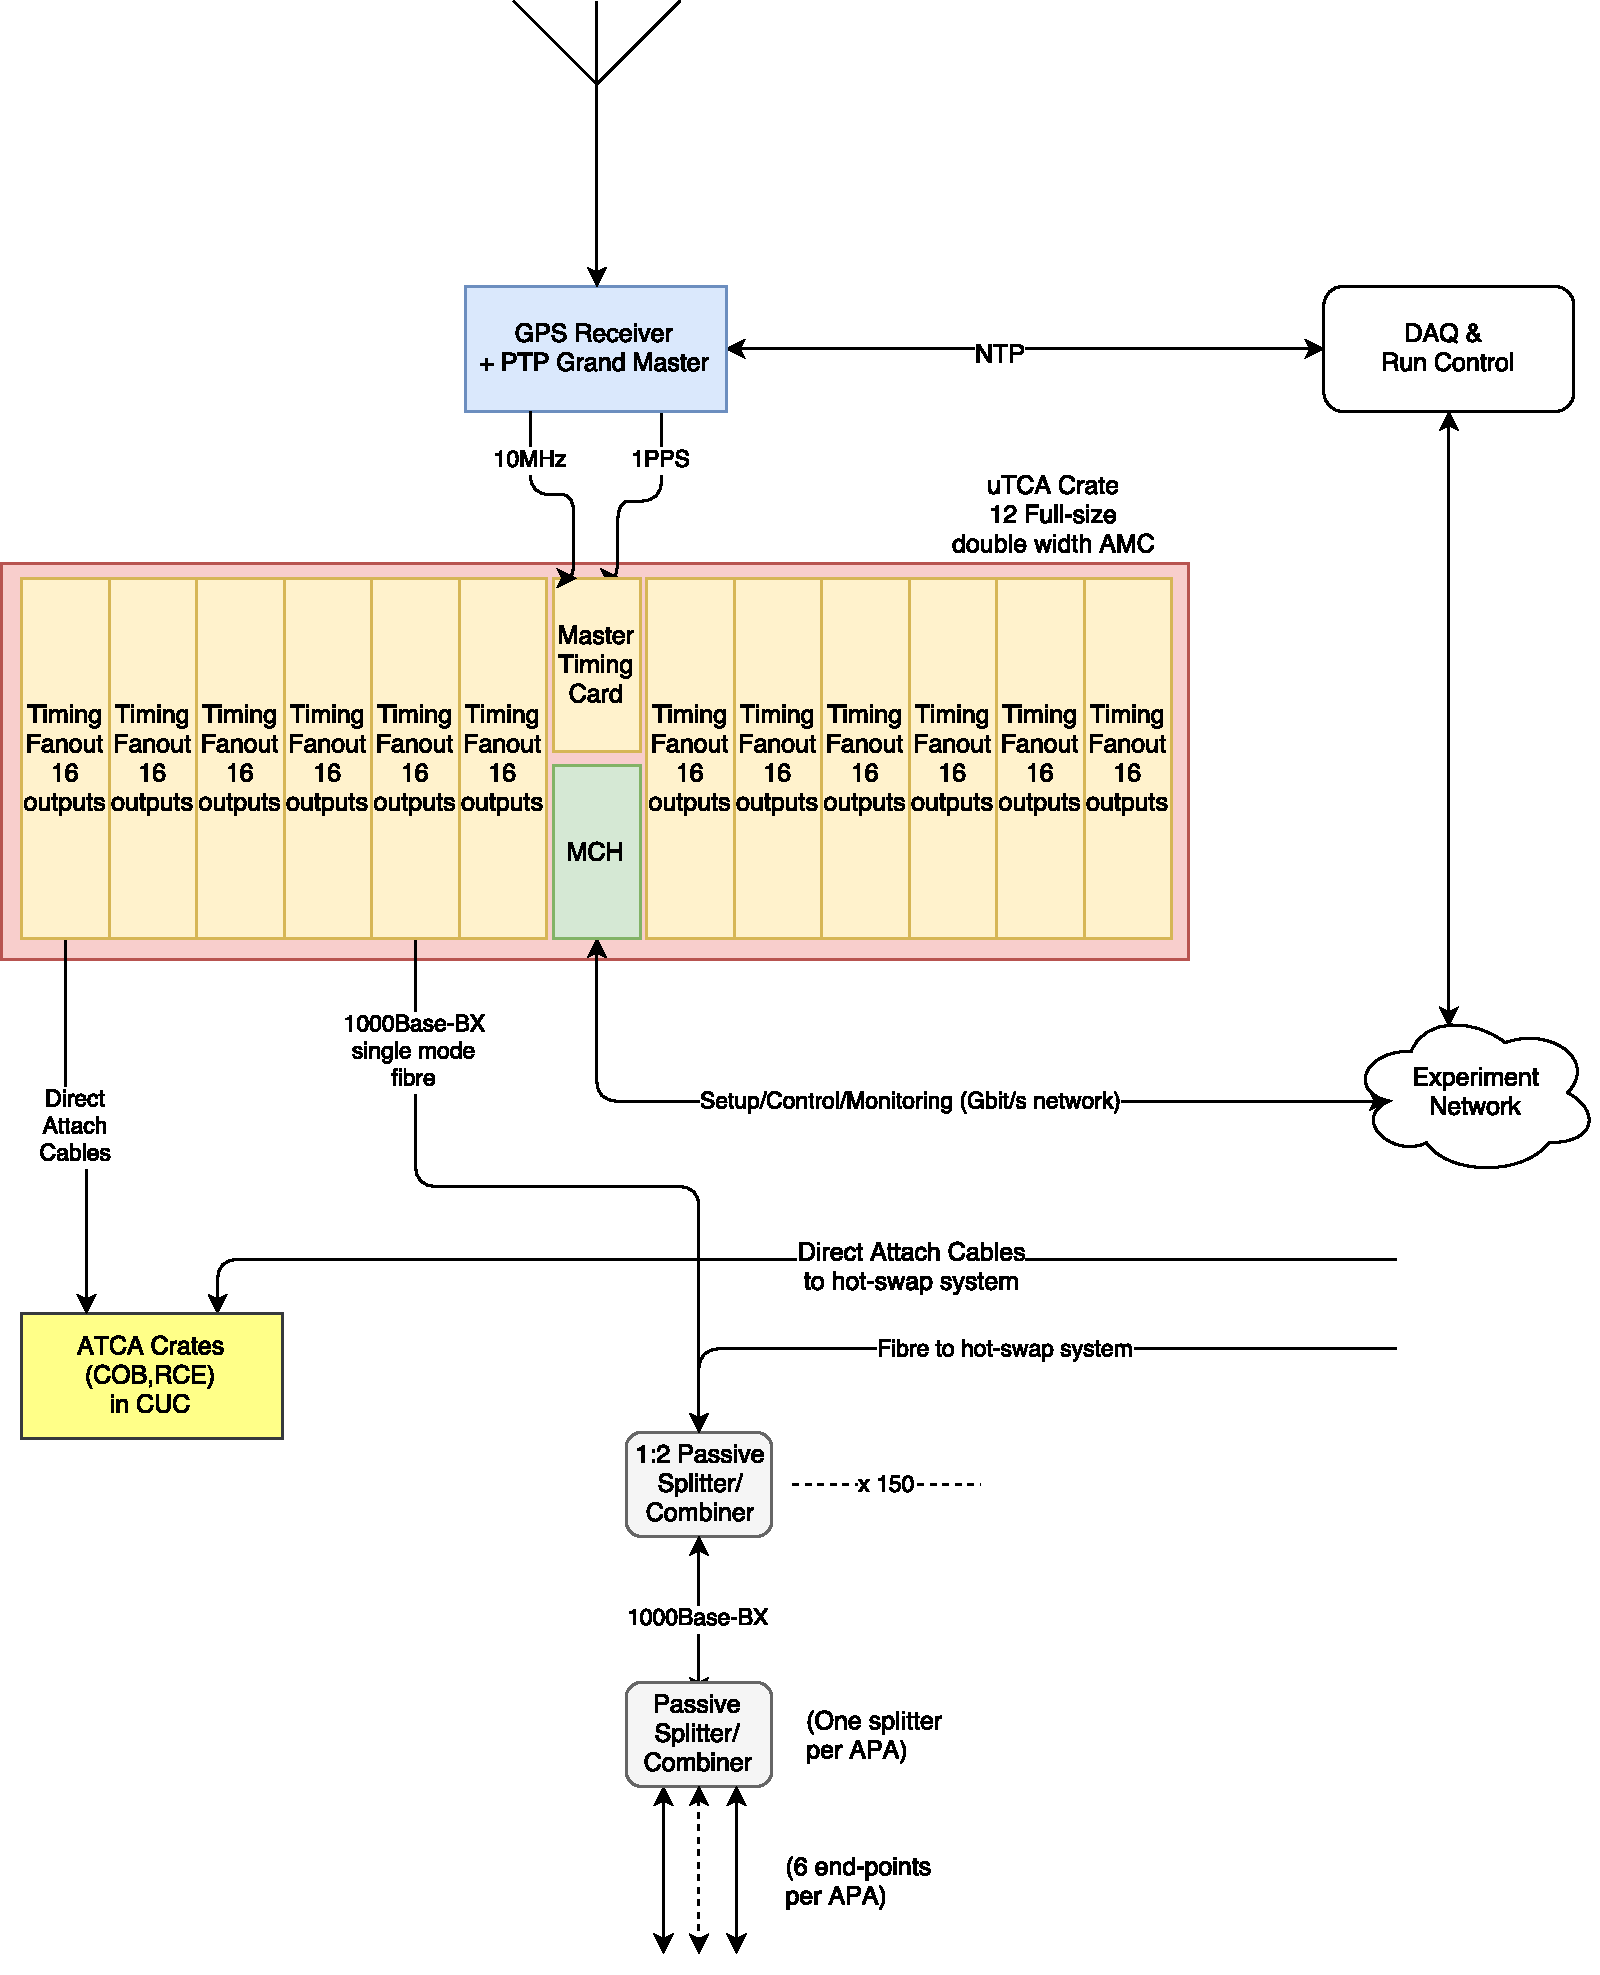
\includegraphics[width=0.8\textwidth]{DUNE_SP_Timing.pdf}
\end{dunefigure}

\subsubsection{Beam timing}
\label{sec:fdsp-daq-design-beamtiming}

The neutrino beam is produced at the Fermilab accelerator complex in
spills of 10$\mu$s duration.  A spill location system (SLS) at the far
detector site will locate the time periods in the data when beam could
be present, based on network packets received from Fermilab containing
preductions of the GPS-time of the spills. data, as it traverses the
DAQ system, where beam intractions may be present.  Experience from
MINOS and NOvA shows that this can provide beam triggering with high
reliability, although the system outlined here contains an extra layer
of reduncancy in this process.  Several stages of narrowing down the
window in which the beam arrives will be done, aiming for an accuracy
of better than 10\% of a drift time, or 0.5\/ms at the time the data
are selected from the DAQ buffers.  Ultimately, an offline database
will match the actual time of the spill with the data, thus removing
any reliance on real-time network transfer for this crucial stage of
the oscillation measurements, the network transfer of spill-timing
information is simply to ensure a correctly located and sufficiently
wide window of data is considered as beam data. This system is not
required, and is not designed to provide signals accurate enough to
measure neutrino time-of-flight.

The precision to which the spill time can be predicted at Fermilab
improves as the acceleration process of the protons producing the
spill in question advances.  The spills currently occur at intervals
of 1.3\/s; the system will be designed to work with any interval, and
to be adaptable in case the sequence described here changes.  For
redundancy, three packets will be sent to the far detector for each
spill.  The first is approximately 1.6\/s before the spill-time, which
is at the point where a 15\/Hz booster cycle is selected; from this
point on, there will be a fixed number of booster cycles until the
neutrinos and the time is subject to a few ms of jitter.  The second
is about 0.7\/s before the spill, at the point where the main injector
acceleration is no longer coupled to the booster timing; this is
governed by a crystal oscillator and so has a few $\mu$s of jitter.
The third will be at the `\$74' which is just before the kicker fires
to direct the protons at the LBNF target; this doesn't improve the
timing at the far detector much, but serves as a cross check for
missing packets.  This system is enhanced compared to that of
MINOS/NOvA, which only use the third of the above timing signals.  The
reason for the larger uncertainty in the time interval from 1.6\/s to
0.7\/s is that the booster cycle time is synchronised to the
electricity supply company's 60\/Hz which has a variation of about
1\%.

Arrival-time monitoring information from a year of MINOS data-taking
was analysed, and it was found that 97\% of packets arrived within
100\/ms of being sent and 99.88\% within 300\/ms.

The spill location system will therefore have estimators of the
GPS-times of future spills, and recent spills contained in the ring
buffers. These estimators will improve in precision as more packets
arrive.  The DAQ will use data in a wider window than usual, if, at
the time the trigger decision has to be made, the precision is less
accurate due to missing or late packets.  From the MINOS monitoting
analysis, this will be very rare.

%%%%%%%%%%%%%%%%%%%%%%%%%%%%%%%%%%%
\subsection{Computing \& Network Infrastructure (Kurt Biery \& Babak Abi)}
\label{sec:fdsp-daq-infra}

Describes the infrastructure that will support the software components described above.

%%%%%%%%%%%%%%%%%%%%%%%%%%%%%%%%%%%
\subsection{Run Control \& Monitoring (Giovanna Miotto \& Jingbo Wang}
\label{sec:fdsp-daq-tcm}

Describe how the system is controlled and monitored.

